\chapter{Radiómica}\label{chap:radiomica}

En este capítulo se presenta el bloque de trabajo basado en radiómica, orientado a transformar las imágenes médicas y sus segmentaciones en un conjunto de características cuantitativas útiles para el análisis y la predicción de complicaciones. Para ello, se describe primero el proceso de extracción de características sobre imágenes originales y preprocesadas, después el análisis exploratorio y la reducción de dimensionalidad aplicada, y finalmente los experimentos de modelado multietiqueta realizados con variables radiómicas y clínicas.


\section{Extracción de características radiómicas}

En esta sección se describe el procedimiento seguido para la extracción de características radiómicas a partir de las imágenes médicas y sus segmentaciones asociadas. El objetivo de esta fase ha sido transformar la información volumétrica contenida en las imágenes en una representación cuantitativa estructurada, utilizable posteriormente en las etapas de análisis, preprocesamiento de variables y modelado predictivo.

La extracción se ha implementado mediante la biblioteca de Python \texttt{PyRadiomics} \cite{van2017computational}, ampliamente utilizada en el análisis de imagen médica para la obtención de descriptores de intensidad, forma y textura, y apoyada en \texttt{SimpleITK} \cite{yaniv2018simpleitk} para el manejo de imágenes médicas y operaciones de remuestreo. Con el fin de mantener la trazabilidad metodológica, esta fase se ha diseñado de forma independiente de la clasificación, de manera que los conjuntos de características pudieran generarse, inspeccionarse y reutilizarse en diferentes experimentos sin acoplar directamente la extracción al entrenamiento de los modelos.

Para todas las variantes evaluadas, el proceso de extracción se ha mantenido bajo una misma configuración de parámetros. En concreto, se han fijado los siguientes ajustes:

\begin{itemize}
    \item \texttt{binWidth = 25}: establece la anchura de los intervalos empleados para discretizar las intensidades antes del cálculo de múltiples características de textura. Este paso resulta relevante porque dichas características no se obtienen directamente a partir de intensidades continuas, sino sobre una versión discretizada de la imagen, por lo que este parámetro influye en el nivel de detalle con el que se representa la heterogeneidad interna de la región analizada.

    \item \texttt{resampledPixelSpacing = [1,1,1]}: permite remuestrear todas las imágenes a un mismo tamaño de vóxel, en este caso isotrópico de 1 mm. De este modo, se reduce la variabilidad asociada a diferencias en la resolución espacial de adquisición y se consigue que las características radiomics se extraigan sobre imágenes espacialmente comparables.
 
    \item \texttt{sitkBSpline}: corresponde al interpolador utilizado durante el remuestreo. Este método permite estimar los nuevos valores de intensidad de forma suave y continua a partir de la información original de la imagen, proporcionando una representación más estable de la estructura radiológica durante el cambio de resolución.

    \item \texttt{normalize}: activa la normalización de intensidades, con el objetivo de homogeneizar la escala global de valores dentro de la región analizada y reducir el efecto de variaciones técnicas entre estudios. De este modo, se favorece que las características extraídas reflejen en mayor medida propiedades del tejido y no únicamente diferencias asociadas a las condiciones de adquisición.

    \item \texttt{removeOutliers = 3}: permite eliminar valores extremos en la distribución de intensidades antes de la normalización. En concreto, se atenúa la influencia de aquellos valores que se desvían más de $\pm 3$ veces la desviación estándar con respecto a la media, evitando que intensidades atípicas afecten de forma desproporcionada al proceso de extracción.
\end{itemize}

En conjunto, esta configuración se ha tomado como referencia para asegurar que las diferencias observadas entre experimentos estuvieran relacionadas principalmente con la región anatómica analizada o con el tipo de imagen de entrada, y no con cambios arbitrarios en el procedimiento de extracción.


Además, conviene distinguir entre los tipos de características que puede generar \texttt{PyRadiomics} y los modos de extracción definidos. De forma general, la biblioteca permite obtener descriptores calculados tanto sobre la imagen original como sobre distintas transformaciones derivadas de ella. Esta posibilidad se ha concretado en dos modos principales. El primero, denominado \textit{basic}, se ha restringido a las características calculadas sobre la imagen original, constituyendo la variante más simple y directamente interpretable. El segundo, denominado \textit{extended}, ha ampliado esta representación incorporando también descriptores obtenidos a partir de imágenes transformadas, con el fin de capturar patrones más complejos de heterogeneidad espacial. En este modo extendido se han incluido, además de la imagen original, transformaciones \textit{Wavelet}, \textit{LoG} con distintos valores de sigma, así como transformaciones \textit{Square}, \textit{SquareRoot}, \textit{Exponential}, \textit{Logarithm}, \textit{Gradient} y descriptores \textit{LBP}. En ambos modos, las características extraídas se han correspondido con los grupos clásicos de \texttt{PyRadiomics}, incluyendo descriptores de primer orden, forma y textura.

A partir de este esquema común, se han desarrollado dos ramas de extracción diferenciadas: una basada en imágenes originales y otra basada en imágenes preprocesadas. Esta separación ha permitido estudiar, por un lado, un escenario de referencia metodológicamente más cercano al planteamiento clásico de la radiómica y, por otro, analizar el posible efecto de distintas transformaciones previas de la imagen sobre las características obtenidas.

\subsection{Extracción sobre imágenes originales}

Una de las estrategias consideradas dentro del bloque radiómico ha sido la extracción de características a partir de las imágenes originales anonimizadas. Esta opción permite trabajar directamente sobre la información tal como se encuentra en los estudios de partida, sin introducir transformaciones previas adicionales que puedan alterar la distribución de intensidades o la estructura espacial de la imagen.

La extracción se ha realizado sobre los volúmenes en formato NIfTI y sus segmentaciones asociadas. En la configuración inicial, la máscara del nódulo se ha considerado la región anatómica principal de interés, al tratarse de la estructura más directamente relacionada con el procedimiento de biopsia. No obstante, el pipeline se ha planteado desde el inicio con la flexibilidad necesaria para incorporar otras máscaras anatómicas y distintas combinaciones entre ellas, de modo que la extracción no quedara restringida a una única región de análisis.

Esta línea de trabajo ha permitido, por tanto, disponer de una representación radiómica obtenida directamente a partir de la imagen original, que posteriormente ha podido compararse con la extraída sobre imágenes preprocesadas para valorar el efecto de ambas estrategias sobre las características generadas y su utilidad en los experimentos de clasificación.

\subsection{Extracción sobre imágenes preprocesadas}

De forma complementaria a la extracción sobre imágenes originales, se ha desarrollado una segunda estrategia basada en imágenes preprocesadas, con el objetivo de analizar si determinadas transformaciones previas podían favorecer la obtención de descriptores radiómicos más informativos. En este caso, el interés no ha residido únicamente en generar nuevas representaciones de la imagen, sino en estudiar de forma comparativa cómo dichas transformaciones podían afectar a la información de intensidad, forma y textura capturada por el proceso de extracción.

Para ello, se han considerado distintas familias de volúmenes preprocesados, incluyendo variantes con redimensionado espacial y variantes derivadas de transformaciones de intensidades basadas en ventanas de unidades Hounsfield. A diferencia de la extracción sobre imágenes originales, en esta rama no se ha trabajado sobre una única colección homogénea de estudios, sino sobre múltiples representaciones generadas a partir de los mismos casos clínicos. Esta circunstancia ha hecho necesario adaptar el pipeline para gestionar de forma sistemática las distintas variantes de entrada, manteniendo en todo momento la correspondencia entre imagen, paciente y máscara anatómica asociada.

La organización de los datos preprocesados también ha diferido del esquema empleado en la extracción sobre imágenes originales, por lo que ha sido necesario desarrollar un extractor específico para este nuevo \textit{layout}. Esta adaptación ha permitido recorrer automáticamente las carpetas de imágenes y máscaras, identificar correctamente las distintas variantes disponibles y generar salidas consistentes y comparables entre preprocesamientos.

Dentro de esta línea, se ha contemplado asimismo la extracción a partir de distintas familias de máscaras anatómicas, incluyendo regiones como pulmón, nódulo, vasos o árbol traqueobronquial. Sin embargo, esta estrategia ha introducido dificultades adicionales relacionadas con la cobertura desigual de algunas máscaras entre pacientes y con la presencia de segmentaciones vacías o no informativas. Estas incidencias se han tratado como un problema de control de calidad del dato, distinguiendo entre la ausencia real de una máscara, la existencia de una máscara sin contenido útil y el fallo efectivo del proceso de extracción.

Además, las variantes \texttt{multiwindowing} han requerido una consideración específica. A diferencia de los volúmenes tridimensionales convencionales, estas representaciones han incorporado varias ventanas como canales diferenciados, generando una estructura efectiva en cuatro dimensiones. Se han separado los canales y se han tratado como imágenes tridimensionales independientes, conservando la geometría espacial correspondiente. Esta solución ha permitido extraer descriptores específicos para cada canal y extender el análisis radiómico a una familia de representaciones que, de otro modo, habría quedado fuera del estudio.

En conjunto, la extracción sobre imágenes preprocesadas ha ampliado el alcance del bloque radiómico, permitiendo comparar distintas formas de representar la imagen antes de la extracción y evaluar hasta qué punto dichas transformaciones influyen en las características obtenidas y en su utilidad posterior para las tareas de clasificación.




\section{Análisis exploratorio y preprocesamiento de las características radiómicas}

Tras la extracción de características radiómicas, se realizó un análisis exploratorio para estudiar la estructura del conjunto de datos, detectar redundancias entre variables y evaluar de forma preliminar su relación con las etiquetas clínicas de complicación.

Como limpieza inicial, se eliminaron metadatos, identificadores, columnas diagnósticas y variables no radiómicas, conservando únicamente las características numéricas válidas para el análisis. Tras este proceso, se obtuvo una matriz de alta dimensionalidad. En el conjunto \textit{basic} se conservaron 214 características, distribuidas de forma equilibrada entre las máscaras de pulmón y nódulo, como se resume en la Tabla~\ref{tab:familias_radiomicas_basic}. La mayor parte de las variables pertenecían a familias de textura y primer orden, como GLCM, GLRLM, GLSZM, GLDM y características estadísticas de intensidad. Por su parte, el conjunto \textit{extended}, al incorporar transformaciones adicionales de la imagen, alcanzó 2961 características, evidenciando un incremento considerable de la dimensionalidad y la necesidad de aplicar técnicas de reducción y selección de variables antes del modelado.

\begin{table}[!htbp]
    \centering
    \small
    \renewcommand{\arraystretch}{1.15}
    \begin{tabular}{lrrr}
        \hline
        \textbf{Familia} & \textbf{Pulmón} & \textbf{Nódulo} & \textbf{Total} \\
        \hline
        First order & 18 & 18 & 36 \\
        GLCM & 24 & 24 & 48 \\
        GLDM & 14 & 14 & 28 \\
        GLRLM & 16 & 16 & 32 \\
        GLSZM & 16 & 16 & 32 \\
        NGTDM & 5 & 5 & 10 \\
        Shape & 14 & 14 & 28 \\
        \hline
        \textbf{Total} & \textbf{107} & \textbf{107} & \textbf{214} \\
        \hline
    \end{tabular}
    \caption{Distribución de características radiómicas \textit{basic} por familia y máscara anatómica.}
    \label{tab:familias_radiomicas_basic}
\end{table}

Desde el punto de vista de la calidad del dato, la presencia de valores nulos en las características radiómicas fue limitada y se debió principalmente a incidencias locales en determinadas máscaras, más que a problemas globales de las imágenes. En algunos pacientes, una región segmentada concreta no contenía una estructura suficientemente definida para extraer características válidas, bien porque la máscara estaba vacía, era demasiado pequeña o presentaba una geometría inadecuada. En otros casos, aparecieron desajustes espaciales puntuales entre la máscara y el volumen de imagen. Como consecuencia, el paciente podía mantenerse en el conjunto de datos, pero el bloque de variables asociado a la máscara afectada quedaba con valores ausentes. En la extracción final fusionada, este fenómeno fue reducido: en las características \textit{basic}, los bloques completos a nulos representaron el 0,49\% en \texttt{lung}, el 1,94\% en \texttt{nodule}, el 0,97\% en \texttt{vessels} y el 1,46\% en \texttt{trachea\_bronchia}. En las características \textit{extended}, los porcentajes fueron del 0,97\%, 2,43\%, 1,46\% y 1,94\%, respectivamente. Por tanto, los valores ausentes se interpretaron como consecuencia de limitaciones locales de segmentación o geometría en máscaras concretas. Tras la limpieza inicial, no se conservaron características completamente vacías ni constantes, y los valores ausentes restantes del bloque numérico fueron imputados mediante la mediana.

La Figura~\ref{fig:eda_radiomics_distribuciones} muestra la distribución de algunas características representativas. Se observa que muchas variables presentan distribuciones asimétricas y con colas largas, especialmente en características de primer orden y textura. Este comportamiento es más acusado en las características asociadas al nódulo, donde algunos descriptores concentran gran parte de los valores cerca de cero y presentan pocos pacientes con valores extremos. Este resultado es relevante porque sugiere la necesidad de aplicar escalado, imputación y selección de variables antes de entrenar modelos predictivos.

\begin{figure}[!htbp]
    \centering
    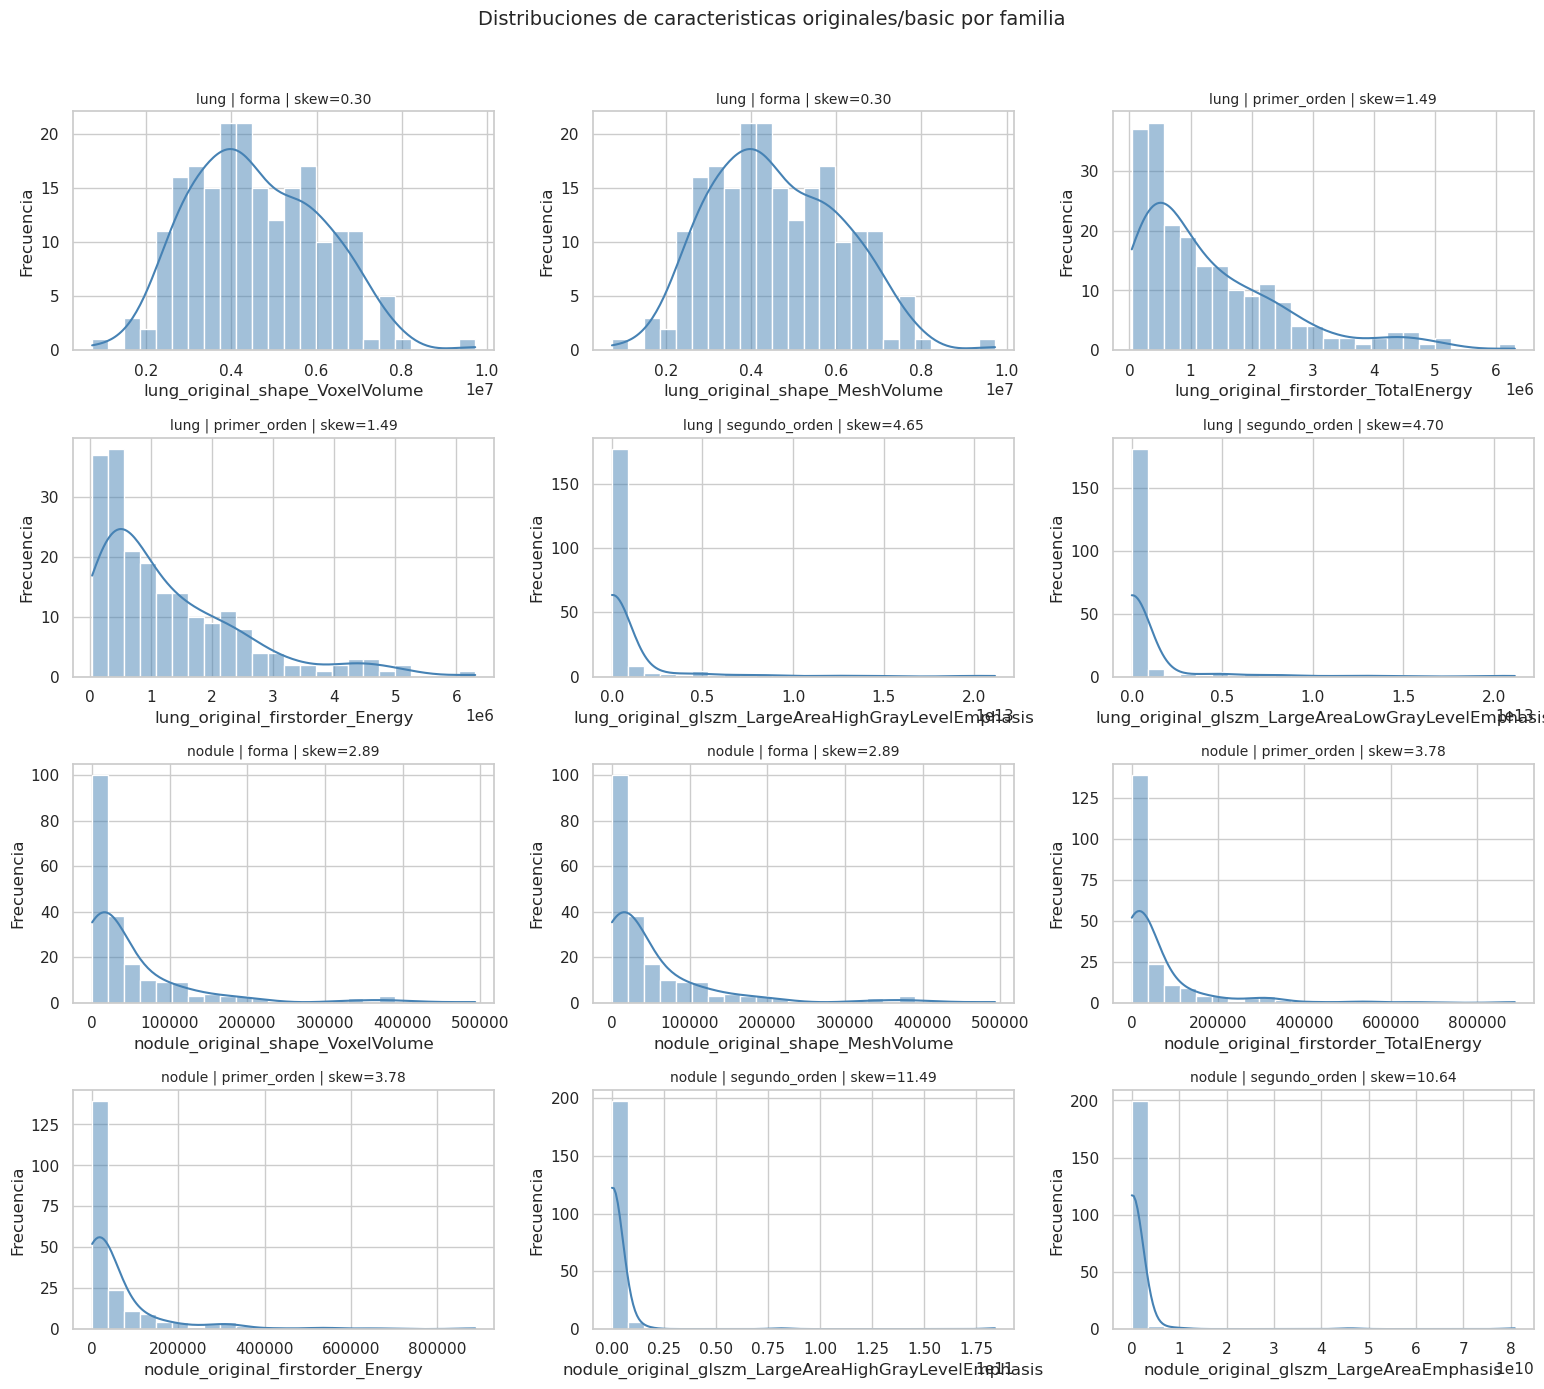
\includegraphics[width=\textwidth]{imagenes/radiomica/eda_radiomics_distribuciones_basic.png}
    \caption{Distribución de características radiómicas originales seleccionadas, separadas por máscara y familia de características.}
    \label{fig:eda_radiomics_distribuciones}
\end{figure}


Uno de los resultados más relevantes del análisis exploratorio fue la elevada dimensionalidad y redundancia de las características radiómicas. Por este motivo, se evaluaron distintas estrategias de reducción no supervisada antes del modelado. En primer lugar, se aplicó \textit{Variance Threshold} con umbral 0,01, con el objetivo de eliminar variables con varianza muy baja. En segundo lugar, se eliminó redundancia lineal descartando características con correlación absoluta superior o igual a 0,95. Finalmente, se estimó el número de componentes principales necesarios para preservar el 90\%, 95\% y 99\% de la varianza mediante PCA. Como se resume en la Tabla~\ref{tab:reduccion_dimensionalidad_radiomics}, el conjunto \textit{basic} se redujo de 214 a 115 características tras eliminar variables redundantes, mientras que el conjunto \textit{extended} pasó de 2961 a 1325. Además, PCA permitió representar el 95\% de la varianza con 26 componentes en el conjunto \textit{basic} y 57 en el conjunto \textit{extended}, lo que indica que gran parte de la información radiómica puede concentrarse en un subespacio de menor dimensión. En el conjunto \textit{multiwindowing basic} seleccionado también se observó una redundancia elevada: 841 de las 1284 características fueron identificadas como redundantes, quedando 443 variables no redundantes.

\begin{table}[!htbp]
    \centering
    \small
    \renewcommand{\arraystretch}{1.15}
    \begin{tabular}{lrr}
        \hline
        \textbf{Etapa} & \textbf{Basic lung+nodule} & \textbf{Extended lung+nodule} \\
        \hline
        Dimensión inicial & 214 & 2961 \\
        \textit{Variance Threshold} 0,01 & 158 & 1312 \\
        Sin redundantes (Corr. $<0,95$) & 115 & 1325 \\
        PCA 90\% & 17 & 32 \\
        PCA 95\% & 26 & 57 \\
        PCA 99\% & 48 & 119 \\
        \hline
    \end{tabular}
    \caption{Reducción de dimensionalidad para los conjuntos de características radiómicas \textit{basic} y \textit{extended}.}
    \label{tab:reduccion_dimensionalidad_radiomics}
\end{table}

Las matrices de correlación antes y después de eliminar variables redundantes se muestran en las Figuras~\ref{fig:eda_radiomics_corr_antes} y~\ref{fig:eda_radiomics_corr_despues}. Estas matrices corresponden al conjunto \textit{basic}, ya que las características \textit{extended} no se presentan debido a su elevada dimensionalidad, que dificultaría la visualización e interpretación del mapa de correlación. Antes del filtrado, se observan bloques de variables altamente correlacionadas, especialmente entre características pertenecientes a la misma familia. Tras aplicar el filtrado por correlación, la estructura queda más dispersa y se reduce de forma notable la presencia de relaciones casi lineales entre variables. Este resultado justifica la eliminación de características redundantes antes del entrenamiento de los modelos, al disminuir la dimensionalidad sin descartar necesariamente información clínica relevante.

\begin{figure}[!htbp]
    \centering
    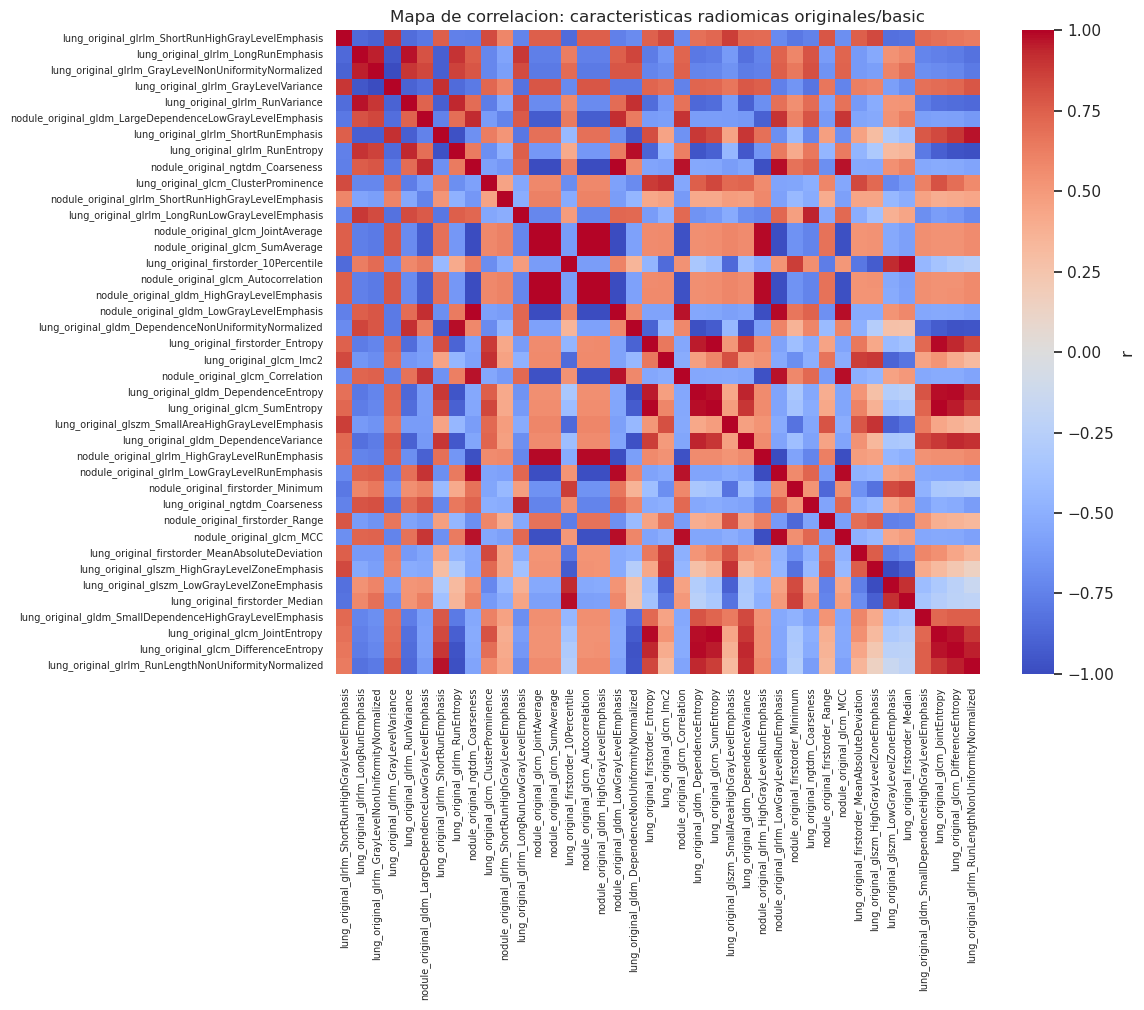
\includegraphics[width=1\textwidth]{imagenes/radiomica/eda_radiomics_corr_basic_antes.png}
    \caption{Matriz de correlación de las características radiómicas originales antes de eliminar variables redundantes.}
    \label{fig:eda_radiomics_corr_antes}
\end{figure}

\begin{figure}[!htbp]
    \centering
    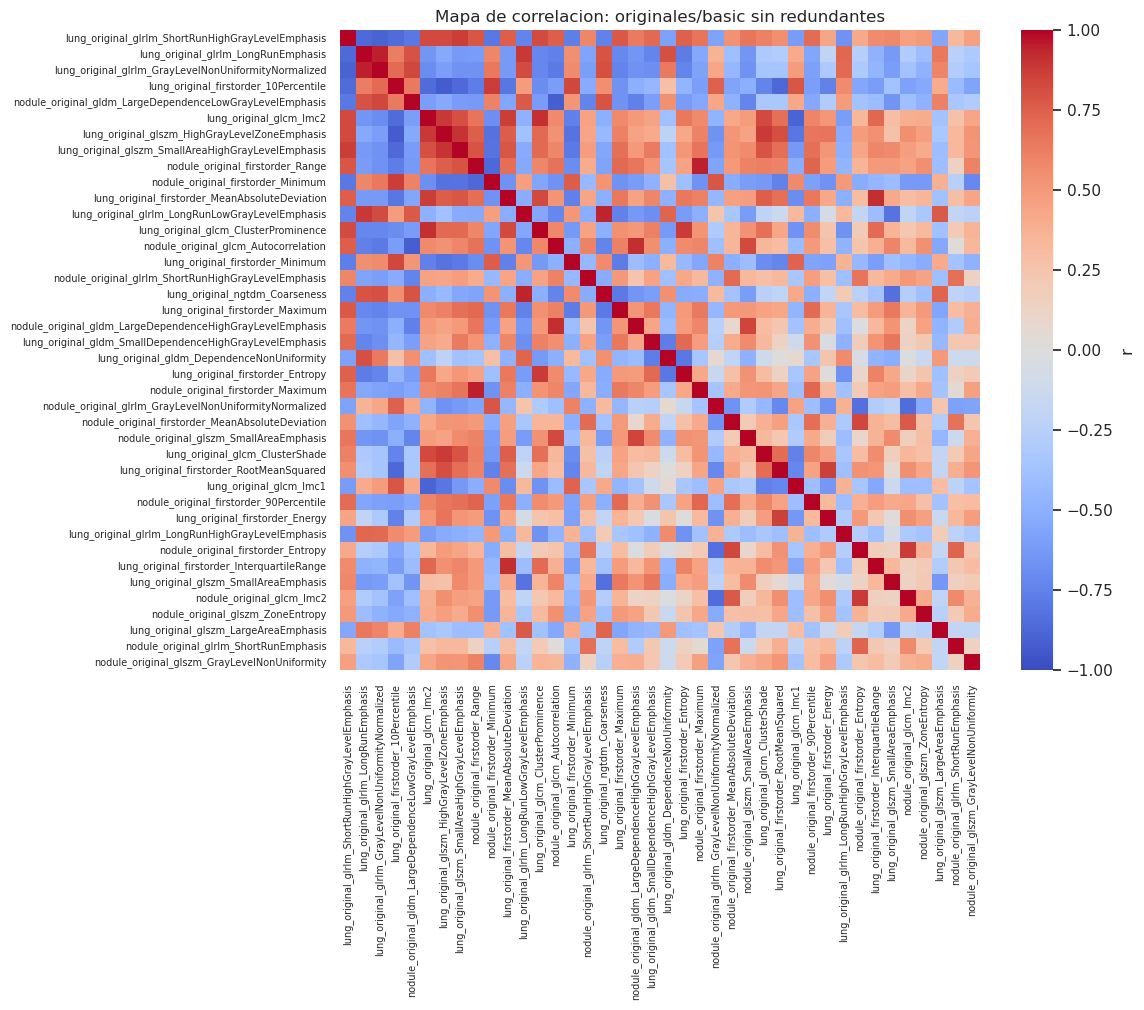
\includegraphics[width=1\textwidth]{imagenes/radiomica/eda_radiomics_corr_basic_despues.png}
    \caption{Matriz de correlación de las características radiómicas tras eliminar variables redundantes mediante filtrado por correlación absoluta superior o igual a 0,95.}
    \label{fig:eda_radiomics_corr_despues}
\end{figure}

La distribución de las correlaciones absolutas por pares, representada en la Figura~\ref{fig:eda_radiomics_distribucion_correlaciones}, confirma esta reducción de redundancia. Aunque la mayor parte de las correlaciones se concentra en valores bajos o moderados, antes del filtrado existe una acumulación clara de pares con correlaciones cercanas a 1. Tras eliminar variables redundantes, esta acumulación se reduce, lo que justifica el uso de este paso como parte del preprocesamiento previo al modelado.

\begin{figure}[!htbp]
    \centering
    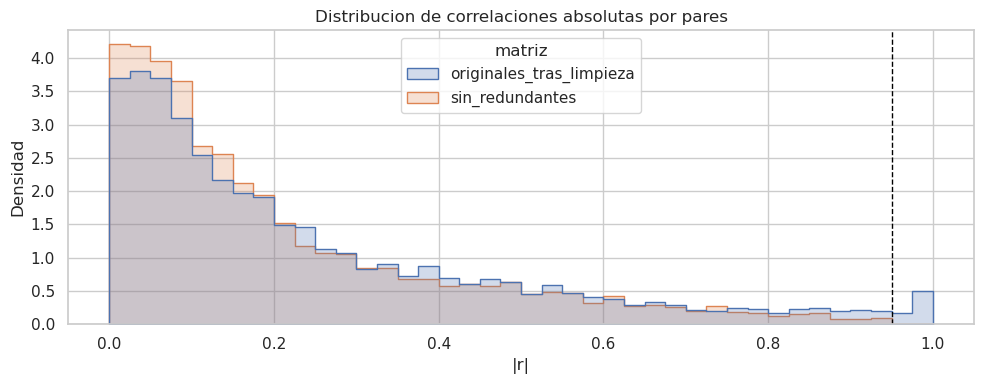
\includegraphics[width=1\textwidth]{imagenes/radiomica/eda_radiomics_distribucion_correlaciones.png}
    \caption{Distribución de correlaciones absolutas entre pares de características antes y después de eliminar variables redundantes.}
    \label{fig:eda_radiomics_distribucion_correlaciones}
\end{figure}

% Respecto a las etiquetas clínicas, el problema mantiene una estructura multietiqueta y presenta un desbalance importante. La etiqueta con mayor soporte es \textit{Sin complicación}, con 105 pacientes, seguida de \textit{Neumotórax}, con 64 casos, y \textit{Hemorragia}, con 49. En cambio, \textit{Derrame pleural} solo aparece en un paciente, por lo que no resulta adecuado extraer conclusiones específicas para esta complicación.

% \begin{table}[!htbp]
%     \centering
%     \small
%     \begin{tabular}{lr}
%         \hline
%         \textbf{Etiqueta} & \textbf{Número de positivos} \\
%         \hline
%         Derrame pleural & 1 \\
%         Hemorragia & 49 \\
%         Neumotórax & 64 \\
%         Sin complicación & 105 \\
%         \hline
%     \end{tabular}
%     \caption{Distribución de etiquetas clínicas empleadas en el análisis radiómico multietiqueta.}
%     \label{tab:etiquetas_radiomics}
% \end{table}

% \begin{figure}[!htbp]
%     \centering
%     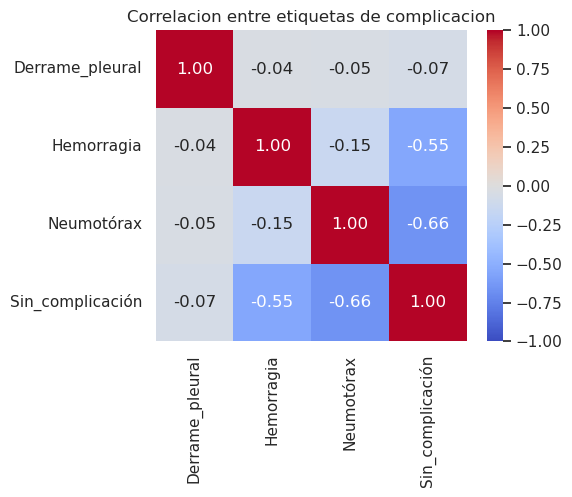
\includegraphics[width=0.75\textwidth]{imagenes/radiomica/eda_radiomics_correlacion_etiquetas.png}
%     \caption{Matriz de correlación entre las etiquetas clínicas de complicación.}
%     \label{fig:eda_radiomics_correlacion_etiquetas}
% \end{figure}

% La relación entre etiquetas clínicas se analizó mediante la matriz de correlación mostrada en la Figura~\ref{fig:eda_radiomics_correlacion_etiquetas}. Como era esperable, la etiqueta \textit{Sin complicación} presenta una correlación negativa con las complicaciones, especialmente con neumotórax y hemorragia. La correlación entre neumotórax y hemorragia también es negativa, lo que indica que, aunque existen pacientes con más de una complicación, ambas etiquetas no tienden a aparecer conjuntamente de forma mayoritaria. En el caso de derrame pleural, el bajo número de positivos impide extraer conclusiones sólidas.

\begin{figure}[!htbp]
    \centering
    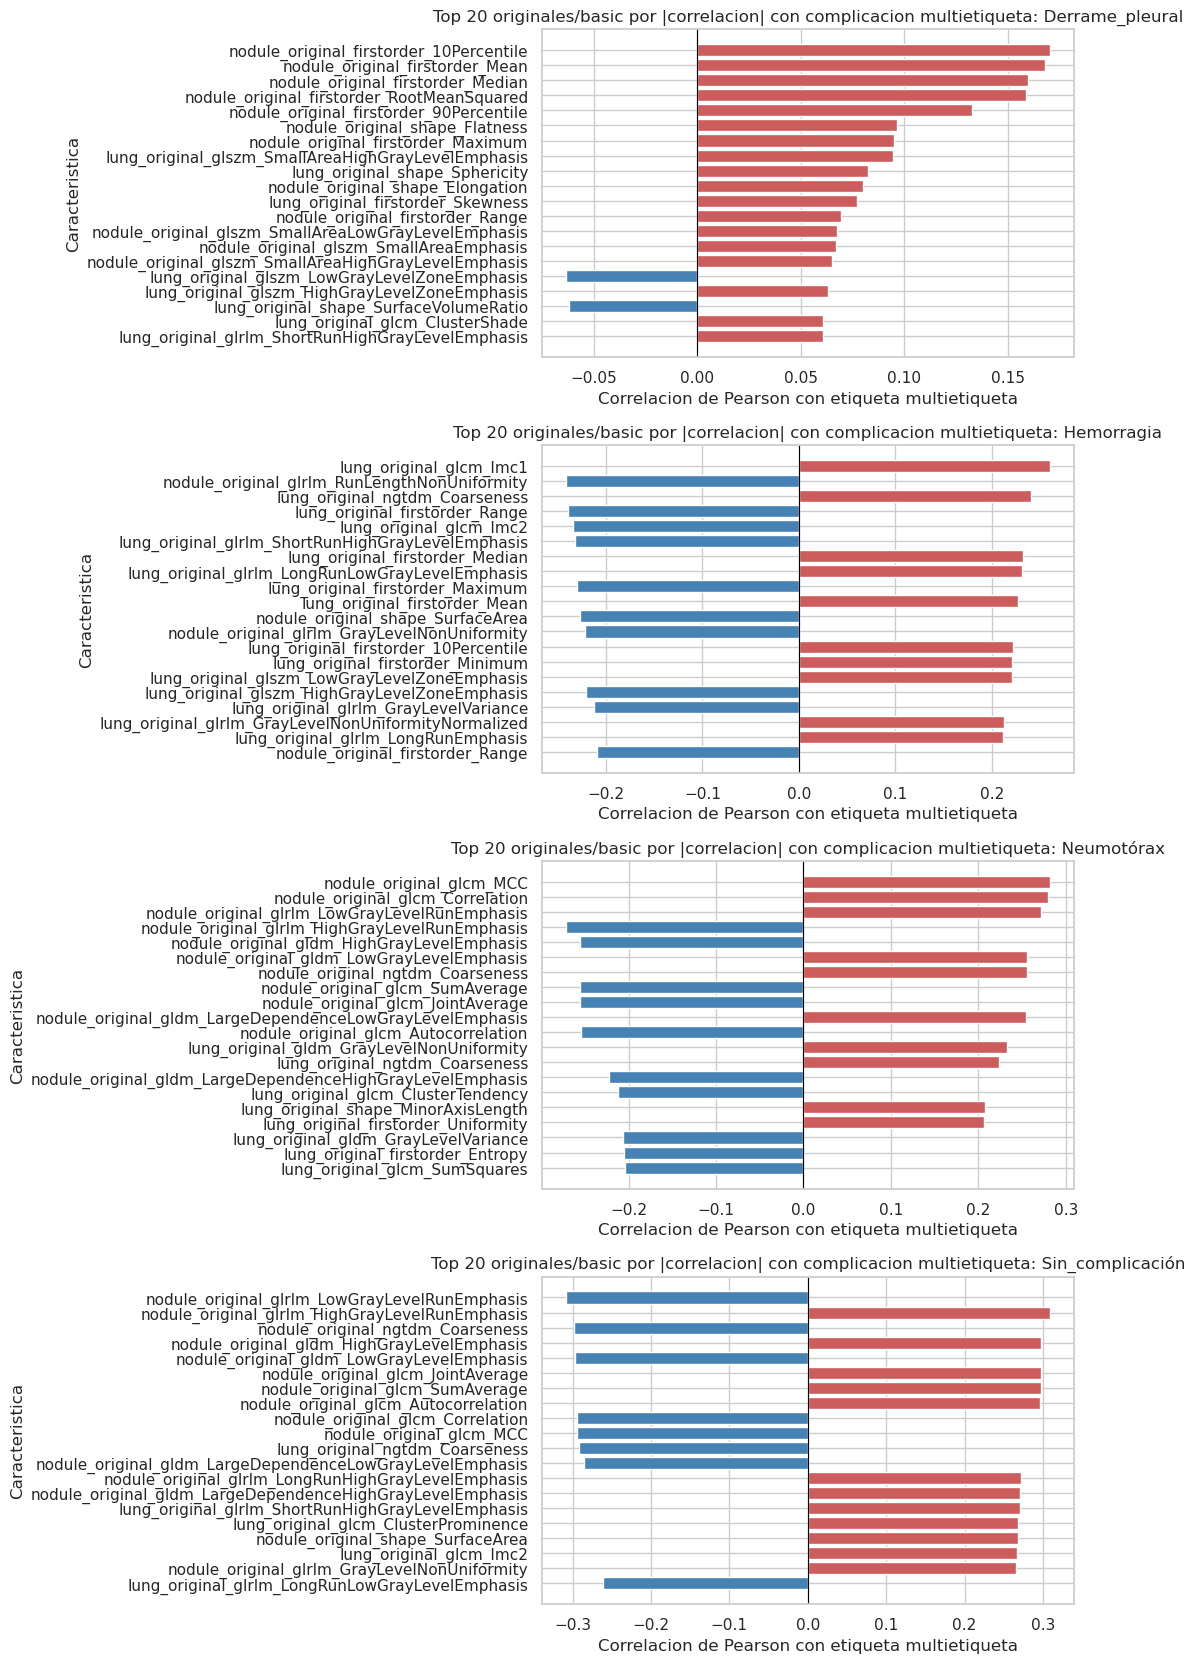
\includegraphics[width=\textwidth]{imagenes/radiomica/eda_radiomics_top_correlaciones_basic.png}
    \caption{Características radiómicas originales o \textit{basic} con mayor correlación absoluta respecto a cada etiqueta clínica de complicación.}
    \label{fig:eda_radiomics_top_correlaciones_basic}
\end{figure}

\begin{figure}[!htbp]
    \centering
    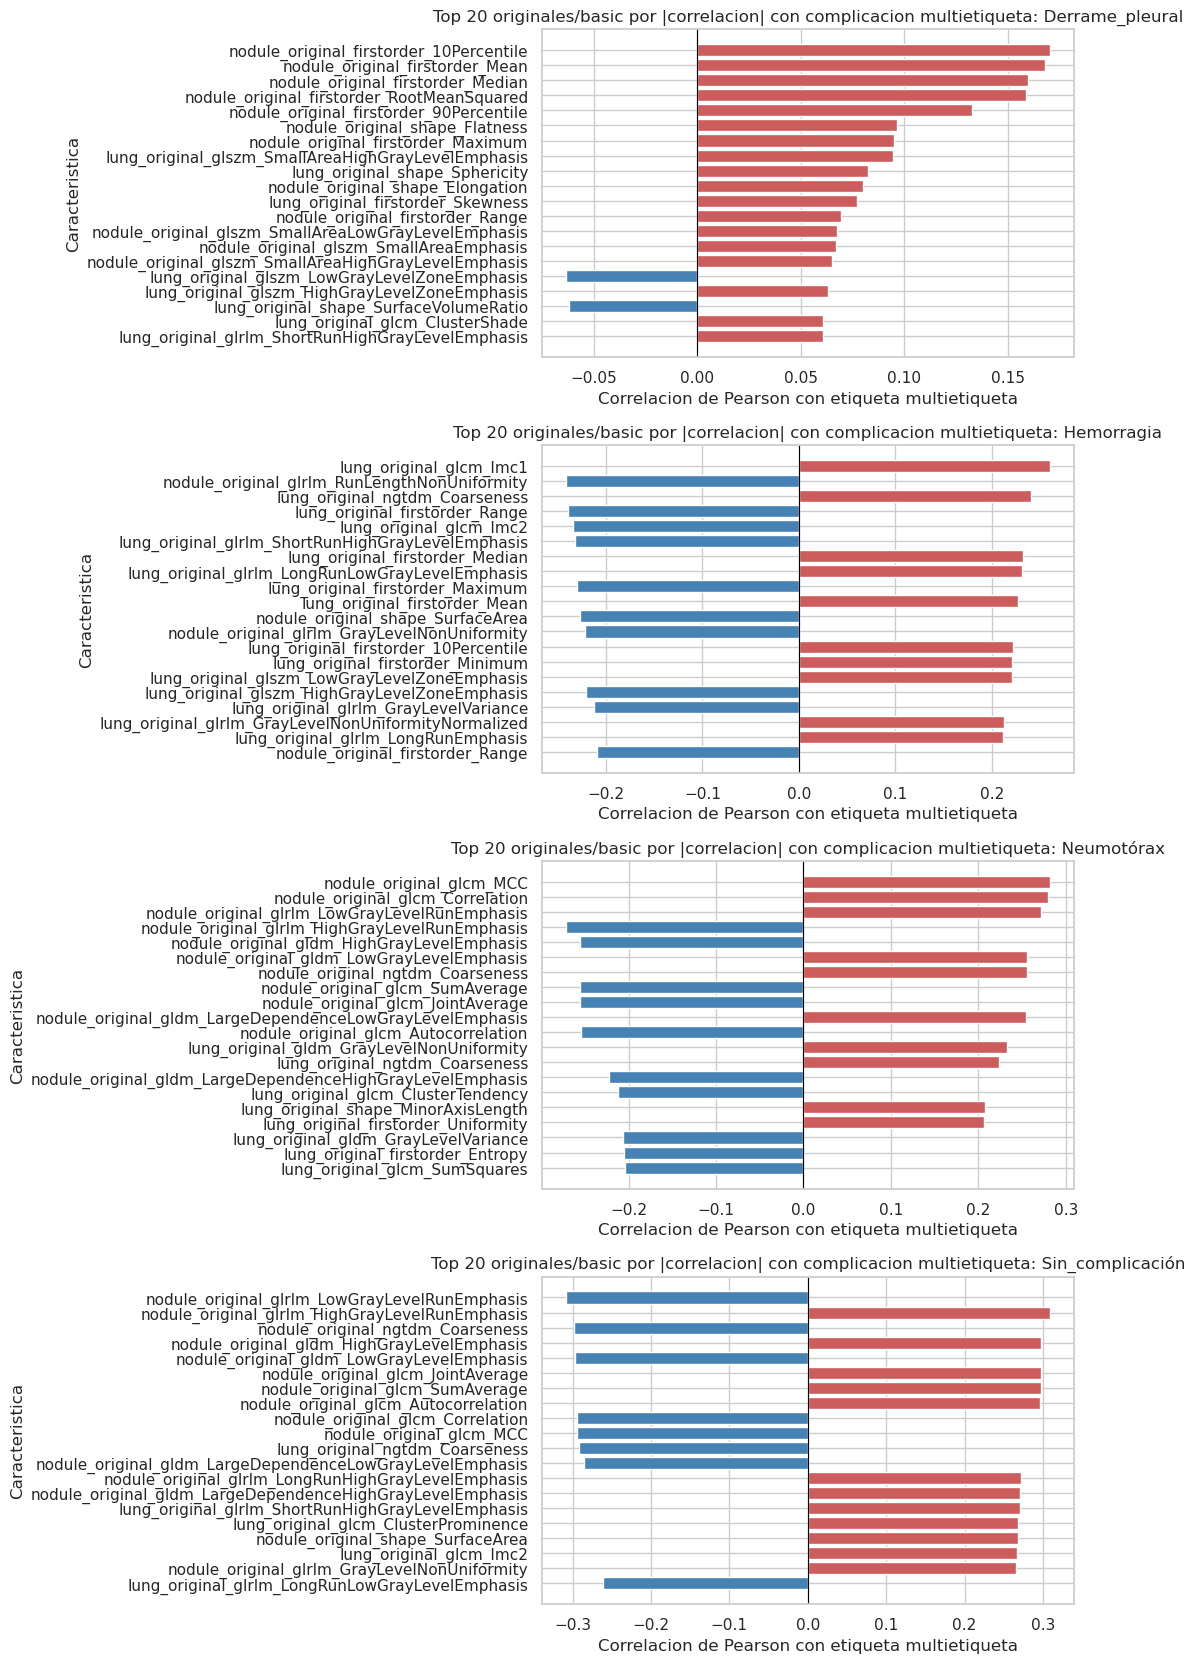
\includegraphics[width=\textwidth]{imagenes/radiomica/eda_radiomics_top_correlaciones_extended.png}
    \caption{Características radiómicas extendidas con mayor correlación absoluta respecto a cada etiqueta clínica de complicación.}
    \label{fig:eda_radiomics_top_correlaciones_extended}
\end{figure}

Finalmente, se analizó la correlación lineal entre las características radiómicas y las etiquetas clínicas de complicación. Para ello, se estudiaron por separado las características originales o \textit{basic} y las características \textit{extended}, como se muestra en las Figuras~\ref{fig:eda_radiomics_top_correlaciones_basic} y~\ref{fig:eda_radiomics_top_correlaciones_extended}. En ambos casos, las correlaciones individuales fueron moderadas, lo que indica que ninguna característica aislada explica por sí sola la aparición de complicaciones. En las características \textit{basic} aparecen descriptores de forma, intensidad y textura tanto del pulmón como del nódulo, mientras que en el conjunto \textit{extended} destacan principalmente variables derivadas de transformaciones como \textit{wavelet}, \textit{log-sigma} o \textit{logarithm}. Este resultado sugiere que la señal predictiva podría estar distribuida entre múltiples descriptores, por lo que el modelado posterior debe apoyarse en técnicas de selección de variables y algoritmos capaces de combinar información débil procedente de distintas familias radiómicas.



\section{Modelado multietiqueta con características radiómicas y clínicas}

Una vez establecida la formulación multietiqueta del problema, se ha abordado el modelado mediante características radiómicas y variables clínicas. Esta aproximación permite evaluar modelos clásicos de aprendizaje automático sobre representaciones tabulares derivadas de la TC, comparando configuraciones basadas únicamente en radiómica, únicamente en información clínica y en la combinación de ambas fuentes.

Como planteamiento principal de modelado se ha trabajado con las complicaciones de mayor interés y soporte muestral suficiente, en particular \textit{Hemorragia} y \textit{Neumotórax}. A partir de ellas, la condición \textit{Sin\_complicación} se ha tratado como una etiqueta derivada, activándose únicamente cuando ninguna de las complicaciones modeladas está presente. De esta forma se evita una formulación redundante o lógicamente inconsistente. También se exploraron formulaciones más amplias con el conjunto completo de etiquetas clínicas disponibles, aunque los resultados de estas variantes fueron menos sólidos cuando alguna complicación presentaba muy pocos casos.

La matriz de entrada se ha construido a nivel de paciente a partir de las características radiómicas extraídas y, cuando ha procedido, se ha ampliado con variables clínicas mediante una unión por identificador. Esto ha permitido comparar de forma homogénea configuraciones de solo radiómica, solo clínica y radiómica más clínica.

Antes del entrenamiento, las variables se han sometido a un preprocesado realizado siempre dentro de cada fold para evitar fuga de información. Este pipeline ha incluido imputación de valores ausentes mediante la mediana, escalado opcional y reducción opcional de dimensionalidad. Entre las estrategias de escalado consideradas se encuentran \texttt{StandardScaler}, \texttt{MinMaxScaler} y la opción de no aplicar escalado cuando la familia de modelos no lo requería. En cuanto a la reducción de dimensionalidad, se han considerado las alternativas \texttt{none}, \texttt{VarianceThreshold} con umbral \(0.01\), y \texttt{PCA} reteniendo el \(90\%\), \(95\%\) o \(99\%\) de la varianza, según la configuración.

Para adaptar clasificadores convencionales al escenario multietiqueta se han considerado tres estrategias de descomposición: \textit{one-vs-rest}, \textit{classifier chain} y \textit{multi-output}. La estrategia \textit{one-vs-rest} permite entrenar un clasificador binario independiente para cada etiqueta; \textit{classifier chain} introduce dependencia secuencial entre etiquetas, lo que puede resultar útil cuando existen relaciones entre complicaciones; y \textit{multi-output} se ha reservado para aquellas familias de modelos en las que esta formulación resultaba directamente compatible.

Sobre este esquema se ha definido un espacio de búsqueda amplio de modelos clásicos. Las familias consideradas en los distintos grids han incluido:

\begin{itemize}
    \item \texttt{LogisticRegression}.
    \item \texttt{SVM} lineal y RBF.
    \item \texttt{KNN}.
    \item \texttt{DecisionTree}.
    \item \texttt{RandomForest}.
    \item \texttt{ExtraTrees}.
    \item \texttt{GradientBoosting}.
    \item \texttt{AdaBoost}.
    \item \texttt{XGBoost}.
    \item \texttt{LightGBM}.
\end{itemize}

De forma exploratoria también se consideraron \texttt{CatBoost} y \texttt{TabPFN}, aunque finalmente no se incorporaron al conjunto principal de experimentos. \texttt{CatBoost} mostraba un coste computacional elevado en algunas configuraciones, mientras que \texttt{TabPFN} presentaba mayores restricciones de aplicación en este problema multietiqueta y con espacios de variables amplios.

Además del clasificador, se exploraron distintas fuentes de características y selecciones de máscaras. Se compararon conjuntos radiómicos \texttt{basic} y \texttt{extended}, variantes derivadas de distintos preprocesados de imagen, configuraciones de solo clínica y combinaciones radiómica más clínica. También se evaluaron máscaras individuales, como \texttt{nodule}, \texttt{lung}, \texttt{vessels} o \texttt{trachea\_bronchia}, y combinaciones con varias regiones como \texttt{lung+nodule}, \texttt{nodule+vessels} o \texttt{lung+nodule+trachea\_bronchia}.

Finalmente, para analizar el efecto del desbalanceo se consideraron medidas como \texttt{class\_weight=balanced}, \texttt{balanced\_subsample} en ensamblados basados en árboles y, en experimentos específicos, sobremuestreo controlado con \texttt{RandomOverSampler} y \texttt{SMOTE}. Estas estrategias se evaluaron sobre configuraciones ya competitivas, en lugar de incorporarse de forma indiscriminada al grid principal.


\section{Análisis experimental de la radiómica}

En esta sección se presenta la experimentación realizada de radiómica, los resultados obtenidos y su interpretación. 

\subsection{Configuracion experimental}

La experimentación radiómica se diseñó para comparar de forma controlada distintas representaciones de entrada, regiones segmentadas, estrategias multietiqueta y combinaciones de modalidades, manteniendo la trazabilidad entre configuración y resultado.

Como base común se trabajó con una cohorte radiómica de 206 pacientes, obtenida a partir de la intersección entre los casos con información clínica disponible y aquellos con imagen y segmentación utilizables. De este modo, las comparaciones entre variantes radiómicas se realizaron sobre la misma cohorte y no quedaron condicionadas por cambios en la composición de pacientes.

A partir de esta cohorte se definió un bloque de referencia con configuraciones radiómicas metodológicamente controladas. Sobre esta base, el diseño experimental se articuló en cuatro ejes principales: tipo de características radiómicas (\texttt{basic} frente a \texttt{extended}), región anatómica segmentada, familia de preprocesado de imagen e incorporación de variables clínicas a la representación de entrada.

\subsection{Validación}

La evaluación de todas las configuraciones se realizó mediante validación cruzada de 5 folds. Según la naturaleza del experimento, se utilizaron particiones \texttt{kfold} o variantes \texttt{labelset\_stratified} cuando la distribución de combinaciones de etiquetas lo permitía. Cuando esta estratificación no era estable por falta de soporte en algunos \textit{labelsets}, se recurrió a un esquema no estratificado.

Para evitar fuga de información, todas las operaciones de preprocesado se ajustaron exclusivamente con los datos de entrenamiento de cada fold y se aplicaron después al subconjunto de validación correspondiente. Esto incluye la imputación de valores ausentes, el escalado, la reducción de dimensionalidad y cualquier transformación de características integrada en el pipeline.

\subsection{Métricas}

Dado el carácter multietiqueta del problema, la evaluación se basó en métricas globales y complementarias.

La métrica principal fue el \textit{F1 micro}, que agrega conjuntamente todas las decisiones binarias del problema y ofrece una visión global del rendimiento:
\[
F1_{\text{micro}} = \frac{2 \, TP}{2 \, TP + FP + FN},
\]
donde \(TP\), \(FP\) y \(FN\) representan, respectivamente, el número total de verdaderos positivos, falsos positivos y falsos negativos acumulados sobre todas las etiquetas.

Como medida complementaria se utilizó el \textit{F1 macro}, que calcula el F1 de cada etiqueta por separado y después obtiene su media aritmética:
\[
F1_{\text{macro}} = \frac{1}{L}\sum_{l=1}^{L} F1_l,
\]

donde \(L\) es el número de etiquetas y \(F1_l\) el valor de F1 para la etiqueta \(l\). Esta métrica resulta útil para valorar el comportamiento medio por complicación y es más sensible al desbalanceo entre etiquetas.

También se consideró la \textit{subset accuracy}, que exige acertar simultáneamente el vector completo de etiquetas de cada paciente:
\[
\text{Subset accuracy} = \frac{1}{N}\sum_{i=1}^{N}\mathbf{1}(\mathbf{y}_i = \hat{\mathbf{y}}_i),
\]
donde \(N\) es el número de pacientes, \(\mathbf{y}_i\) es el vector real de etiquetas y \(\hat{\mathbf{y}}_i\) el vector predicho.

La \textit{Hamming loss} cuantifica la proporción de etiquetas mal clasificadas:
\[
\text{Hamming loss} = \frac{1}{N \cdot L}\sum_{i=1}^{N}\sum_{l=1}^{L}\mathbf{1}(y_{il} \neq \hat{y}_{il}).
\]
A diferencia de la \textit{subset accuracy}, esta métrica penaliza error por error y no exige acertar todo el vector de etiquetas a la vez.

De forma adicional se analizaron \textit{precision micro}, \textit{recall micro}, \textit{Jaccard micro} y métricas por etiqueta.

La \textit{precision micro} mide la proporción de predicciones positivas correctas sobre el total de predicciones positivas realizadas:
\[
\text{Precision}_{\text{micro}} = \frac{TP}{TP + FP}.
\]

La \textit{recall micro} mide la proporción de positivos reales que el modelo consigue recuperar:
\[
\text{Recall}_{\text{micro}} = \frac{TP}{TP + FN}.
\]

Por su parte, el \textit{Jaccard micro} cuantifica la coincidencia global entre etiquetas reales y predichas:
\[
\text{Jaccard}_{\text{micro}} = \frac{TP}{TP + FP + FN}.
\]

En estas expresiones, \(TP\), \(FP\) y \(FN\) representan los verdaderos positivos, falsos positivos y falsos negativos acumulados sobre todas las etiquetas.

Además, se calcularon métricas por etiqueta, evaluando cada complicación de forma independiente. Para una etiqueta \(l\), la precisión, la exhaustividad y la puntuación F1 se definen como:
\[
\text{Precision}_l = \frac{TP_l}{TP_l + FP_l}, \qquad
\text{Recall}_l = \frac{TP_l}{TP_l + FN_l},
\]
\[
F1_l = \frac{2 \cdot \text{Precision}_l \cdot \text{Recall}_l}{\text{Precision}_l + \text{Recall}_l}.
\]

Este análisis permitió detectar configuraciones con buen comportamiento global, pero con bajo rendimiento en alguna complicación concreta.

\subsection{Descripción de los experimentos}

El diseño experimental distinguió entre experimentos principales y exploratorios. Los experimentos principales se centraron en formulaciones con soporte muestral suficiente y en configuraciones con coste computacional razonable. En cambio, las extensiones a espacios de búsqueda más amplios, combinaciones de máscaras más complejas o familias adicionales de modelos se interpretaron como análisis exploratorios.

En conjunto, la experimentación no se planteó como un barrido indiscriminado, sino como una secuencia de comparaciones controladas. Primero se estableció una referencia reproducible sobre la cohorte común; después se evaluó el efecto del tipo de características y de la región segmentada; posteriormente se compararon distintos preprocesados; y, por último, se analizaron extensiones como la incorporación de variables clínicas o el tratamiento específico del desbalanceo.

\subsection{Resultados y análisis}

A partir de los experimentos, los mejores resultados globales se concentraron en un conjunto reducido de configuraciones con rendimiento muy similar. 

La Tabla~\ref{tab:top_modelos_radiomica} resume las configuraciones con mejor rendimiento global ordenadas por \textit{F1 micro}. El mejor resultado correspondió a una configuración basada en características \texttt{extended}, preprocesado $(128,128,128)$ y ventana HU $[-1350,150]$, combinación de máscaras de pulmón, nódulo, tráquea y bronquios, y modelo \textit{XGBoost}, con un \textit{F1 micro} de 0.6222. Muy cerca aparecen varias configuraciones con \textit{ExtraTrees} sobre representaciones más simples, especialmente con máscara \texttt{nodule} o con la combinación \texttt{lung+nodule}, lo que indica que el mejor rendimiento no depende de una única elección de modelo o de una única representación de entrada.

En conjunto, los resultados muestran dos patrones principales. En primer lugar, los modelos basados en árboles dominan claramente las primeras posiciones, con presencia repetida de \textit{XGBoost}, \textit{ExtraTrees}, \textit{GradientBoosting} y \textit{LightGBM}. En segundo lugar, las diferencias entre configuraciones son pequeñas: los mejores valores de \textit{F1 micro} se concentran aproximadamente entre 0.61 y 0.62, con \textit{subset accuracy} en torno a 0.58-0.61 y \textit{Hamming loss} alrededor de 0.26. Esto sugiere que existe un techo de rendimiento relativamente estable y que, dentro del espacio evaluado, los cambios de modelo, escalado o reducción de dimensionalidad producen mejoras limitadas.

También se observa que las configuraciones mejor posicionadas no siguen un único patrón de complejidad. Algunas de las mejores combinaciones utilizan características \texttt{extended} y máscaras multirregión, pero otras muy competitivas se apoyan en representaciones \texttt{basic} y en la máscara \texttt{nodule} de forma aislada. Esto sugiere que aumentar la cantidad de información de entrada no garantiza por sí mismo una mejora clara, probablemente porque el tamaño muestral es reducido en relación con la dimensionalidad del problema y porque no toda la información añadida resulta igualmente discriminativa.

El hecho de que el mejor \textit{F1 micro} apenas supere 0.62 indica que la capacidad predictiva del enfoque es moderada. Este comportamiento puede explicarse por varios factores. En primer lugar, la cohorte disponible para modelado sigue siendo pequeña para un problema multietiqueta con alta dimensionalidad, lo que limita la estabilidad de los modelos y favorece la variabilidad entre folds. En segundo lugar, las complicaciones no solo son infrecuentes, sino también heterogéneas desde el punto de vista clínico y radiológico, de modo que la relación entre radiómica preprocedimiento y evento postbiopsia probablemente sea débil o indirecta en muchos casos. En tercer lugar, parte de la señal relevante puede no estar completamente contenida en las características radiómicas extraídas, sino depender también de factores técnicos y clínicos del procedimiento, como la localización exacta de la lesión, la trayectoria de la aguja, la profundidad, la cercanía a estructuras vasculares o antecedentes funcionales del paciente.

Además, la formulación multietiqueta añade dificultad adicional respecto a un problema binario simple. El modelo no solo debe detectar la presencia de complicación, sino distinguir entre tipos de complicación potencialmente solapados y con frecuencias desiguales. Esto ayuda a explicar que métricas más exigentes, como la \textit{subset accuracy}, se mantengan alrededor de 0.60 incluso en las mejores configuraciones. Del mismo modo, la diferencia sistemática entre \textit{F1 micro} y \textit{F1 macro} indica que el rendimiento no es uniforme entre etiquetas y que las clases menos favorecidas siguen siendo más difíciles de modelar.

En consecuencia, aunque estos resultados permiten identificar combinaciones metodológicas más competitivas que otras, no muestran una separación fuerte entre configuraciones ni evidencian un modelo claramente dominante.

\begin{landscape}
\begin{table}[p]
\centering
\tiny
\setlength{\tabcolsep}{1.3pt}
\renewcommand{\arraystretch}{0.85}

\begin{adjustbox}{max width=\linewidth, max height=0.88\textheight, keepaspectratio}
\begin{tabular}{l l l l l l l r r r r r r r}
\hline
Preprocesado & Features & Máscaras & Modelo & Scaler & Red. dim. & Parámetros & F1 micro & F1 macro & Subset acc. & Hamming loss & Jaccard micro & Precision micro & Recall micro \\
\hline
(128,128,128) HU [-1350,150] & extended & lung+nodule+trachea\_bronchia & XGBoost & none & none & lr=0.1, depth=5, n=100 & 0.6222 & 0.5263 & 0.6098 & 0.2585 & 0.4534 & 0.6324 & 0.6125 \\
(128,128,128) original & basic & nodule & ExtraTrees & none & none & depth=10, n=100, minsplit=5 & 0.6201 & 0.5392 & 0.6000 & 0.2581 & 0.4531 & 0.6381 & 0.6032 \\
(128,128,128) original & basic & lung+nodule & ExtraTrees & none & none & depth=10, n=200, minsplit=2 & 0.6190 & 0.5339 & 0.5854 & 0.2585 & 0.4503 & 0.6366 & 0.6030 \\
(128,128,128) original & basic & nodule & ExtraTrees & minmax & none & depth=10, n=50, minsplit=5 & 0.6189 & 0.5332 & 0.6000 & 0.2598 & 0.4504 & 0.6356 & 0.6032 \\
(128,128,128) original & basic & nodule & ExtraTrees & none & none & depth=10, n=50, minsplit=5 & 0.6189 & 0.5332 & 0.6000 & 0.2598 & 0.4504 & 0.6356 & 0.6032 \\
(128,128,128) HU [-1350,150] & extended & lung+nodule+trachea\_bronchia & XGBoost & none & none & lr=0.1, depth=10, n=100 & 0.6174 & 0.5139 & 0.6049 & 0.2618 & 0.4488 & 0.6276 & 0.6079 \\
(sin ventana HU explícita) & basic & lung+nodule+vessels & GradientBoosting & none & varth\_0.01 & lr=0.1, depth=3, n=200 & 0.6164 & 0.5711 & 0.6000 & 0.2650 & - & 0.6207 & 0.6122 \\
(sin ventana HU explícita) & basic & lung+nodule+vessels & GradientBoosting & none & varth\_0.01 & lr=0.1, depth=3, n=200 & 0.6164 & 0.5711 & 0.6000 & 0.2650 & - & 0.6207 & 0.6122 \\
(128,128,128) HU [-1350,150] & extended & lung+nodule+trachea\_bronchia & XGBoost & minmax & none & lr=0.1, depth=10, n=100 & 0.6160 & 0.5125 & 0.6000 & 0.2634 & 0.4473 & 0.6247 & 0.6079 \\
(128,128,128) HU [-1350,150] & extended & lung+nodule+trachea\_bronchia & XGBoost & std & none & lr=0.1, depth=10, n=100 & 0.6160 & 0.5125 & 0.6000 & 0.2634 & 0.4473 & 0.6247 & 0.6079 \\
(sin ventana HU explícita) & basic & lung+nodule+vessels & GradientBoosting & none & varth\_0.01 & lr=0.03, depth=3, n=400 & 0.6151 & 0.5615 & 0.5805 & 0.2667 & - & 0.6180 & 0.6123 \\
(sin ventana HU explícita) & basic & lung+nodule+vessels & GradientBoosting & none & varth\_0.01 & lr=0.03, depth=3, n=400 & 0.6151 & 0.5615 & 0.5805 & 0.2667 & - & 0.6180 & 0.6123 \\
(sin ventana HU explícita) & basic & vessels & LightGBM & none & varth\_0.01 & lr=0.1, depth=6, n=700, leaves=31 & 0.6146 & 0.5239 & 0.5854 & 0.2650 & - & 0.6219 & 0.6078 \\
(128,128,128) HU [-1350,150] & extended & lung+nodule+trachea\_bronchia & XGBoost & std & none & lr=0.01, depth=5, n=200 & 0.6143 & 0.4817 & 0.6049 & 0.2634 & 0.4445 & 0.6261 & 0.6030 \\
(128,128,128) HU [-1350,150] & extended & lung+nodule+trachea\_bronchia & XGBoost & minmax & none & lr=0.1, depth=5, n=100 & 0.6127 & 0.5156 & 0.6000 & 0.2650 & 0.4440 & 0.6227 & 0.6032 \\
(128,128,128) HU [-1350,150] & extended & lung+nodule+trachea\_bronchia & XGBoost & std & none & lr=0.1, depth=5, n=100 & 0.6127 & 0.5156 & 0.6000 & 0.2650 & 0.4440 & 0.6227 & 0.6032 \\
(128,128,128) original & basic & lung+nodule & ExtraTrees & std & none & depth=10, n=100, minsplit=2 & 0.6121 & 0.5252 & 0.5756 & 0.2618 & 0.4432 & 0.6322 & 0.5937 \\
(128,128,128) original & basic & lung+nodule & ExtraTrees & minmax & none & depth=10, n=100, minsplit=2 & 0.6120 & 0.5257 & 0.5756 & 0.2618 & 0.4425 & 0.6319 & 0.5937 \\
(128,128,128) original & basic & nodule & ExtraTrees & minmax & none & depth=10, n=100, minsplit=5 & 0.6118 & 0.5341 & 0.5897 & 0.2650 & 0.4449 & 0.6261 & 0.5983 \\
(128,128,128) original & basic & lung+nodule & ExtraTrees & none & none & depth=10, n=100, minsplit=2 & 0.6112 & 0.5259 & 0.5707 & 0.2650 & 0.4419 & 0.6251 & 0.5982 \\
(sin ventana HU explícita) & extended & lung+nodule+vessels & XGBoost & none & varth\_0.01 & lr=0.03, depth=6, n=700 & 0.6112 & 0.5205 & 0.5805 & 0.2699 & - & 0.6146 & 0.6080 \\
(sin ventana HU explícita) & extended & lung+nodule+vessels & XGBoost & none & varth\_0.01 & lr=0.03, depth=6, n=700 & 0.6112 & 0.5205 & 0.5805 & 0.2699 & - & 0.6146 & 0.6080 \\
(128,128,128) original & basic & nodule & ExtraTrees & std & none & depth=10, n=50, minsplit=5 & 0.6104 & 0.5159 & 0.5949 & 0.2650 & 0.4418 & 0.6285 & 0.5934 \\
(128,128,128) HU [-1350,150] & extended & lung+nodule+trachea\_bronchia & XGBoost & minmax & none & lr=0.01, depth=5, n=200 & 0.6095 & 0.4726 & 0.6000 & 0.2667 & 0.4398 & 0.6213 & 0.5983 \\
(128,128,128) HU [-1350,150] & extended & lung+nodule+trachea\_bronchia & XGBoost & none & none & lr=0.01, depth=5, n=200 & 0.6095 & 0.4726 & 0.6000 & 0.2667 & 0.4398 & 0.6213 & 0.5983 \\
(128,128,128) HU [-1000,400] & basic & lung+nodule+trachea\_bronchia+vessels & LightGBM & minmax & none & lr=0.1, n=200, leaves=31 & 0.6084 & 0.5209 & 0.5902 & 0.2699 & 0.4393 & 0.6142 & 0.6032 \\
(128,128,128) HU [-1000,400] & basic & lung+nodule+trachea\_bronchia+vessels & LightGBM & minmax & none & lr=0.1, n=200, leaves=50 & 0.6084 & 0.5209 & 0.5902 & 0.2699 & 0.4393 & 0.6142 & 0.6032 \\
(sin ventana HU explícita) & basic & nodule+vessels & LightGBM & none & varth\_0.01 & lr=0.03, depth=6, n=300, leaves=31 & 0.6082 & 0.5021 & 0.5805 & 0.2683 & - & 0.6188 & 0.5981 \\
(sin ventana HU explícita) & extended & lung+nodule+vessels & XGBoost & none & varth\_0.01 & lr=0.03, depth=6, n=700 & 0.6077 & 0.5237 & 0.5805 & 0.2715 & - & 0.6123 & 0.6033 \\
(128,128,128) HU [-1350,150] & extended & lung+nodule+trachea\_bronchia & XGBoost & std & none & lr=0.01, n=200 & 0.6063 & 0.4678 & 0.6000 & 0.2683 & 0.4360 & 0.6195 & 0.5936 \\
\hline
\end{tabular}
\end{adjustbox}

\caption{Mejores configuraciones obtenidas en los experimentos de clasificación multietiqueta con estrategia \textit{chain}, ordenadas de mayor a menor F1 micro.}
\label{tab:top_modelos_radiomica}
\end{table}
\end{landscape}
